\chapter{Estado del Arte}
\section{Técnicas de Aprendizaje Colaborativo}

\subsection{La técnica de Jigsaw}

La técnica de Jigsaw, que fue introducida por \citeA{aronson_jigsaw_1978} para mejorar la cooperación en pares y crear solidaridad en equipo entre los estudiantes a través de la división de tareas, involucra a cada estudiantes en un grupo a asumir responsabilidades en el aprendizaje. En consecuencia, los estudiantes trabajan en dos diferentes grupos: el grupo de expertos y el grupo jigsaw.\\

Los objetivos de está técnica son:

\begin{itemize}
  \item Estructurar las interacciones entre los alumnos, mediante equipos de trabajo.
  \item Lograr que los alumnos dependan unos de otros para lograr sus objetivos.
\end{itemize}

La secuencia de pasos que conforman esta técnica son los siguientes \footnote{\cite{upm_2008}}:

\begin{enumerate}
  \item El docente debe tener preparada la división del tema a tratar en cinco o séis documentos, los cuales se repartirán a los alumnos siguiendo un orden. Cada uno de ellos será necesario para aprender la totalidad del tema, y por lo tanto, todos ellos formarán la unidad temática completa.
  \item Se divide a los alumnos en grupos de cinco o séis(según el número de documentos elaborados) y dentro de cada grupo cada miembro recibirá un número de 1 a 5(ó 6). Ver figura \ref{fig:jigsaw01}

\begin{figure}[h]
  \centering
  % Requires \usepackage{graphicx}
  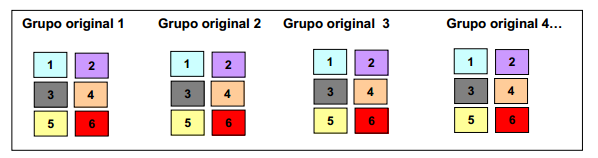
\includegraphics[scale=0.6]{figuras/jigsaw01.png}\\
  \caption{Grupos originales en la técnica Jigsaw}\label{fig:jigsaw01}
\end{figure}

A los estudiantes con el número 1 se les reparte el mismo documento, que será diferente al resto de los compañeros y que puede corresponderse a la primera parte del tema de estudio. A los alumnos con el número 2 se les reparte otro documento y así sucesivamente.

La primera fase será, por tanto, que los alumnos preparen su documento de forma individual, que lo lean, que lo entienda, que lo aprendan y que recopilen las dudas que surjan.

  \item Una vez que ya ha finalizado el tiempo estimado para la preparación individual del documento, comienta la segunda fase que se denomina ``Reunión de expertos''. En este momento todos los alumnos con el mismo número se reúnen para debatir y comentar sobre el documento que les fue asignado. Ver figura \ref{fig:jigsaw02}

  \begin{figure}[h]
  \centering
  % Requires \usepackage{graphicx}
  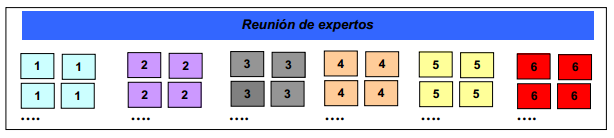
\includegraphics[scale=0.6]{figuras/jigsaw02.png}\\
  \caption{Grupos de expertos}\label{fig:jigsaw02}
\end{figure}

    \item Finalizada las reuniones de expertos, llega la tercera fase, que supone el regreso al grupo original y, cada alumno explicará al resto de sus compañeros el documentos que ha estado preparando. Ver figura \ref{fig:jigsaw03}

\begin{figure}[h]
  \centering
  % Requires \usepackage{graphicx}
  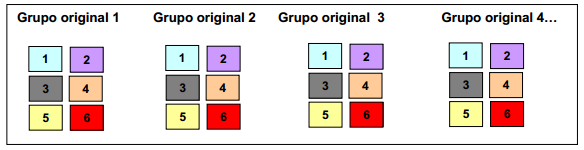
\includegraphics[scale=0.6]{figuras/jigsaw03.png}\\
  \caption{Regreso a los originales}\label{fig:jigsaw03}
\end{figure}

\item La última fase, consiste en evaluar el aprendizaje logrado y la eficacia de la técnica individualmente. Para ello, el docente prepara un test sobre todo el material que ha sido trabajado durante la sesión de clase.

\end{enumerate}

\subsection{Programación en pares}
Una técnica educacional que tiene elementos en común con el aprendizaje cooperativo es la programación en pares. En esta forma de colaboración, dos programadores trabajan lado a lado en un computador. En cualquier momento, un miembro del equipo(``the driver'') está escribiendo en el computador o transcribiendo algún diseño elaborado. El otro integrante del equipo (``the navigator'') está observando activamente el trabajo del primero, buscando defectos, pensando en otras alternativas de solución, haciendo preguntas, etc. Los roles de ``driver'' y ``navigator'' son intercambiados periódicamente entre ambos miembros del equipo.\\

La programación en pares fue originalmente popularizada como parte de la metodología de desarrollo de software XP \cite{beck_extreme_2000}. Así mismo, resultados de investigaciones muestran que los programadores en pares producen código de mayor calidad en mitad de tiempo que lo programadores individuales \cite{williams2000collaborative,williams_strengthening_2000}. La técnica de programación en pares también has mostrado ser efectiva para estudiantes de programación, logrando mejorar el aprendizaje en los alumnos\cite{mcdowell_effects_2002}.

\subsection{El estudio de Casos}
Es una técnica de aprendizaje cooperativo, la cual está basada en un enfoque de estudio de problemas. \cite{JCAL:JCAL119}. Durante un Estudio de Casos, los estudiantes reciben materiales que describen una situación en concreto y se les pide analizarla tratando de identificar los puntos fuertes y débiles del caso, así como también se les pide reflexionar sobre posibles soluciones que pudiesen añadir a las ya presentadas en el problema. El factor más importante del Estudio de Casos es que éstos están basados en problemas y/o situaciones reales \cite{JCAL:JCAL119}.


\subsection{Técnicas para el diálogo}
\subsection{Técnicas para la enseñanza recíproca}
\subsubsection{Celdas de aprendizaje}
\subsubsection{La pecera}
\subsubsection{Juego de rol}
\subsubsection{Jigsaw - Rompecabezas}
\subsubsection{Equipo de exámenes}
\subsection{Técnicas para la resolución de problemas}

\section{Aplicaciones web de tiempo real}
\subsection{Qué es tiempo real}
El término tiempo real se refiere a la naturaleza oportuna entre la ocurrencia de un evento y el ser advertidos de ello. La medición en el tiempo entre un evento ocurrido y la entrega de ese evento depende en realidad del evento. Si el evento es la aplicación del pie al frenar un auto, entonces el tiempo entre el pie bajando y los frenos que se aplica tiene que ser absolutamente mínimo. Sin embargo, si el evento es el envío de un mensaje de chat en un foro de fútbol y se muestra a los demás usuarios, es poco probable hacer una gran diferencia de unos segundos. En último caso, el evento tiene que ser entregado en un tiempo suficientemente corto. Si te cortas un dedo, no hay retraso entre el corte y el registro de dolor. Esto es tiempo real. Sin embargo, la posibilidad de desarrollar tiempo real no era inicialmente algo fácil. Pero los desarrolladores han llegado a soluciones inteligentes y ``hacks'' para resolver el problema de comunicación entre el servidor y el cliente.

\subsubsection{AJAX}
Cuando el JavaScript empezó a ser más relevante, los desarrolladores empezaron a mejorar el nivel de los objetos XMLHttpRequest para enviar peticiones HTTP de forma asíncrona, o sin necesidad de refrescar la página web actual. Esto fue llamado AJAX(Asynchronous JavaScript and XML).\\

Ajax, es una tecnología usada en aplicaciones Web 2.0 que está basada en JavaScript y con la cual se puede obtener data del lado del servidor para actualizar parcialmente el contenido de una página\cite{wang_design_2014}.

\subsubsection{Polling}
Después del posicionamiento de AJAX, no pasó mucho tiempo para tratar de lograr que los eventos en el navegador salieran fuera de la ecuación y automatizar el proceso de obtener nueva información. Fue entonces que los desarrolladores establecieron un intervalo de actualización para revisar actualizaciones cada $n$ segundos. Ver figura \ref{fig:polling}
\begin{figure}[h]
  \centering
  % Requires \usepackage{graphicx}
  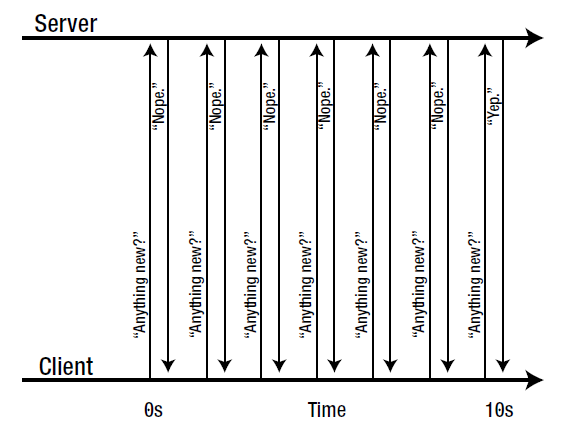
\includegraphics[scale=0.8]{figuras/polling.png}\\
  \caption{Polling envía peticiones HTTP para comprobar si existe nueva información}\label{fig:polling}
\end{figure}

\subsubsection{HTTP Long-Polling}
El siguiente paso en la evolución del tiempo real es el HTTP \emph{long-polling}, el cual consiste en abrir una petición HTTP por un periodo de tiempo para escuchar respuestas del servidor. Si hubiese nueva data, el servidor la enviaría y se cerraría la petición; de otro modo, la petición es cerrada después de un intervalo de tiempo límite y se abre una nueva petición. Ver figura \ref{fig:http_long_polling}
\begin{figure}[h]
  \centering
  % Requires \usepackage{graphicx}
  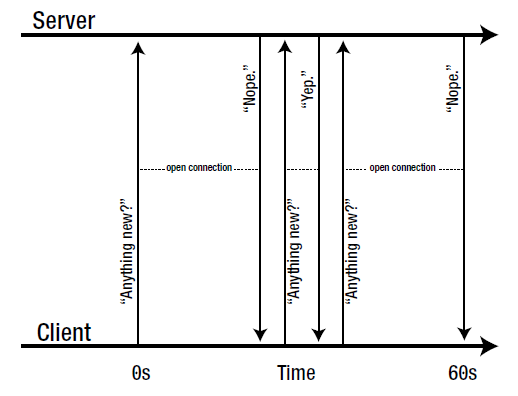
\includegraphics[scale=0.8]{figuras/http_long_polling.png}\\
  \caption{HTTP Long-polling mantiene abierta una peticion HTTP por un periodo de tiempo para comprobar si existe nueva información}\label{fig:http_long_polling}
\end{figure}
%%\cite{lengstorf2013realtime}

\subsubsection{HTTP Streaming}
HTTP Streaming es muy similar a HTTP long-polling, excepto que la conexión no es cerrada cuando hay nueva información o se vence el intervalo de tiempo. En lugar de ello, la nueva data se envía sobre la conexión que permanece abierta.

\subsubsection{Comet}
Es un modelo de aplicación web en el que una petición HTTP mantenida abierta permite al servidor web enviar datos al cliente sin que éste los solicite explícitamente.

\subsubsection{WebSockets}
Web sockets es una tecnología que proporciona un canal de comunicación bidireccional y full-duplex sobre una única conexión TCP en los navegadores y servidores web. A comparación de HTTP, WebSocket puede reducir efectivamente el tráfico de red innecesario, a través de una forma estandarizada para que el servidor envíe contenido al navegador sin que éste sea solicitado.\cite{cheng_new_2013}
